\documentclass[mat1, tisk]{fmfdelo}
\usepackage{amsmath}
\usepackage{graphicx}
\usepackage{hyperref}
% \documentclass[fin1, tisk]{fmfdelo}
% Če pobrišete možnost tisk, bodo povezave obarvane,
% na začetku pa ne bo praznih strani po naslovu, …

%%%%%%%%%%%%%%%%%%%%%%%%%%%%%%%%%%%%%%%%%%%%%%%%%%%%%%%%%%%%%%%%%%%%%%%%%%%%%%%
% METAPODATKI
%%%%%%%%%%%%%%%%%%%%%%%%%%%%%%%%%%%%%%%%%%%%%%%%%%%%%%%%%%%%%%%%%%%%%%%%%%%%%%%

% - vaše ime
\avtor{Manca Murn}

% - naslov dela v slovenščini
\naslov{Metrična dimenzija leksikografskega produkta grafov}

% - naslov dela v angleščini
\title{The metric dimension of the lexicographic product of graphs}

% - ime mentorja/mentorice s polnim nazivom:
%   - doc.~dr.~Ime Priimek
%   - izr.~prof.~dr.~Ime Priimek
%   - prof.~dr.~Ime Priimek
%   za druge variante uporabite ustrezne ukaze
\mentor{Sandi Klavžar}
% \somentor{...}
% \mentorica{...}
% \somentorica{...}
% \mentorja{...}{...}
% \somentorja{...}{...}
% \mentorici{...}{...}
% \somentorici{...}{...}

% - leto diplome
\letnica{2023} 

% - povzetek v slovenščini
%   V povzetku na kratko opišite vsebinske rezultate dela. Sem ne sodi razlaga
%   organizacije dela, torej v katerem razdelku je kaj, pač pa le opis vsebine.
\povzetek{...}

% - povzetek v angleščini
\abstract{... }

% - klasifikacijske oznake, ločene z vejicami
%   Oznake, ki opisujejo področje dela, so dostopne na strani https://www.ams.org/msc/
\klasifikacija{..., ...}

% - ključne besede, ki nastopajo v delu, ločene s \sep
\kljucnebesede{...\sep ...}

% - angleški prevod ključnih besed
\keywords{...\sep ...} % angleški prevod ključnih besed

% - angleško-slovenski slovar strokovnih izrazov
\slovar{
% \geslo{angleški izraz}{slovenski izraz}
% ...
}

% - ime datoteke z viri (vključno s končnico .bib), če uporabljate BibTeX
% \literatura{....bib}

%%%%%%%%%%%%%%%%%%%%%%%%%%%%%%%%%%%%%%%%%%%%%%%%%%%%%%%%%%%%%%%%%%%%%%%%%%%%%%%
% DODATNE DEFINICIJE
%%%%%%%%%%%%%%%%%%%%%%%%%%%%%%%%%%%%%%%%%%%%%%%%%%%%%%%%%%%%%%%%%%%%%%%%%%%%%%%

% naložite dodatne pakete, ki jih potrebujete
% \usepackage{...}

% deklarirajte vse matematične operatorje, da jih bo LaTeX pravilno stavil
% \DeclareMathOperator{\...}{...}

% vstavite svoje definicije ...
% \newcommand{\...}{...}


%%%%%%%%%%%%%%%%%%%%%%%%%%%%%%%%%%%%%%%%%%%%%%%%%%%%%%%%%%%%%%%%%%%%%%%%%%%%%%%
% ZAČETEK VSEBINE
%%%%%%%%%%%%%%%%%%%%%%%%%%%%%%%%%%%%%%%%%%%%%%%%%%%%%%%%%%%%%%%%%%%%%%%%%%%%%%%

\begin{document}

\section{Uvod}
V decembru leta 2010 sta v razmaku 17 dni nastala dva različna članka z enakim naslovom - 
\textit{"The metric dimension of the lexicographic product of graphs"}. Avtorji obeh člankov 
bojda niso vedeli za delo drugega in so se teme lotili na dva posvem različna načina. 
V tem diplomskem seminarju si bomo ogledali pojem metrične dimenzije grafa in njene osnovne 
lastnosti, definirali leksikografski produkt grafov ter povzeli glavne rezultate o metrični 
dimenziji leksikografskega produkta iz obeh člankov. Na koncu bomo skušali najti tudi 
povezavo med enim in drugim pristopom obravnave le te. 


%%%%%%%%%%%%%%%%%%%%%%%%%%%%%%%%%%%%%%%%%%%%%%%%%%%%%%%%%%%%%%%%%%%%%%%%%%%%%%%
%%%%%%%%%%%%%%%%%%%%%%%%%%%%%%%%%%%%%%%%%%%%%%%%%%%%%%%%%%%%%%%%%%%%%%%%%%%%%%%


\subsection{Osnovni pojmi}
Za začetek ponovimo nekaj osnovnih definicij in oznak iz teorije grafov, ki jih bomo potrebovali 
za razumevanje tega diplomskega seminarja. 

\begin{definicija}
    Graf $G$ je urejen par $(V(G), E(G)),$ kjer je $V(G)$ množica vozlišč in $E(G)$ 
    podmnožica v $\binom{V(G)}{2},$ ki vsebuje povezave grafa.
\end{definicija}

Če je $V(G)$ končna množica, je $G$ končen graf. Če je med dvema različnima vozliščema največ 
ena povezava in nobeno vozlišče ni povezano samo s seboj, pravimo, da je graf enostaven. 
Vozlišči $v, u \in G$ sta sosedni, če $uv \in E(G).$ Sosednost je ekvivalenčna relacija, zato 
sosedni vozlišči označimo $u \sim v.$ Če $w, x \in V(G)$ nista sosedni pa pišemo $w \not \sim x.$

\begin{definicija}
    Komplement grafa $G$, je graf $\overline{G},$ za katerega velja $V(G) = V(\overline{G})$ in 
    $$\forall u,v \in V(\overline{G}): uv E(\overline{G}) \Leftrightarrow uv \not \in E(G).$$
\end{definicija}

Sprehod v grafu $G$ je zaporedje vozlišč $v_1, v_2, ... v_k$ iz $V(G)$, tako da je 
$\forall i : v_i, v_{i+1} \in E(G).$ Sprehod je enostaven, če vsebuje sama različna vozlišča.
Graf je povezan, če med vsakima dvema različnima vozliščema obstaja sprehod. Na povezanem
grafu lahko definiramo razdaljo med vozliščema.

\begin{definicija}
    Razdalja med dvema vozliščema $u, v \in V(G)$ je dolžina najkrajšega sprehoda in jo 
    označujemo z $d(u, v).$ 
\end{definicija}

Naslednja trditev o razdaji med vozlišči je očitna.

\begin{trditev} \label{nicelna_razdalja}
    Za povezan graf $G$ in poljubni vozlišči $v, w \in V(G)$ velja:
    $$ d(v, w) = 0 \Leftrightarrow v=w.$$
\end{trditev} 

\begin{definicija}
    Graf $H$ je podgraf grafa $G$ natanko tedaj, ko velja $V(H) \subseteq V(G)$ in 
    $E(H) \subseteq E(H)$.
\end{definicija}

\begin{definicija}
    Graf $H$ je induciran podgraf grafa $G$ natanko tedaj, ko velja 
    $\forall u, v \in V(H) : uv \in E(G) \Rightarrow E(H)$.
\end{definicija}

\begin{definicija}
Komponenta grafa je povezan podgraf, ki ni del nobenega večjega povezanega podgrafa. 
\end{definicija}

Povezan graf ima seveda samo eno komponento. Definirajmo še operacijo združitve grafov.

\begin{definicija}
    Združitev grafov $G$ in $H$, je graf $G + H$, za katerega velja $V(G + H) = V(G) \cup V(H)$ 
    in $E(G + H)  = E(G) \cup E(H) \cup \{ uv \;  | \;  u \in V(G) \land v \in V(H) \}.$
\end{definicija}
% ali je ta definicija ok? In prevod... ne najdem sploh definicije za joint graphs.

Poglejmo še nekaj primerov osnovnih razredov grafov:
\begin{itemize}
    \item Polni graf na $n$ vozliščih, ki ga označujemo z $K_n$, ima vse možne povezave.
    \item Polni dvodelni graf, ki ga označujemo z $K_{n, m}$ ima množico 
    vozlišč $V(K_{n,m}) = \{ v_1, v_2, ... , v_n , u_1, u_2, ... , u_m \}$
    in povezave $E(K_{n, m}) = \{ v_i u_j \; | 1 \leq i \leq n \land 1 \leq j \leq m \}.$ 
    \item Pot na $n$ vozliščih, ki jo označujemo z $P_n$, ima množico povezav 
    $E(P_n) = \{ v_1 v_2 , v_2 v_3 , ... , v_{n-1} v_n\}.$
    \item Cikel na $n$ vozliščih, dobimo tako, da grafu $P_n$ dodamo povezavo $n 1$.
    \item Drevo je povezan graf, ki ne vsebuje nobenega cikla.
\end{itemize}


%%%%%%%%%%%%%%%%%%%%%%%%%%%%%%%%%%%%%%%%%%%%%%%%%%%%%%%%%%%%%%%%%%%%%%%%%%%%%%%
%%%%%%%%%%%%%%%%%%%%%%%%%%%%%%%%%%%%%%%%%%%%%%%%%%%%%%%%%%%%%%%%%%%%%%%%%%%%%%%
%%%%%%%%%%%%%%%%%%%%%%%%%%%%%%%%%%%%%%%%%%%%%%%%%%%%%%%%%%%%%%%%%%%%%%%%%%%%%%%
%%%%%%%%%%%%%%%%%%%%%%%%%%%%%%%%%%%%%%%%%%%%%%%%%%%%%%%%%%%%%%%%%%%%%%%%%%%%%%%


\section{Metrična dimenzija grafa}

%motivacija neki izvirnega

\subsection{Definicija}

Metrična dimenzija grafa je najmanjše število vozlišč grafa, ki jih potrebujemo, da
vsa vozlišča v grafu razlikujemo med sabo zgolj s pomočjo razdalj do izbranih vozlišč.
V matematičnem jeziku to povemo takole:

\begin{definicija} \label{def:1}
    Naj bo $G$ povezan graf in $W = \{ w_1, ... , w_k  \} \subseteq V(G)$ neprazna 
    podmnožica vozlišč. Vektor $r_W(v) = (d(v, w_1), ..., d(v, w_k))$ imenujemo metrična 
    predstavitev vozlišča $v \in V(G)$ s podmnožico $W$.
\end{definicija}

\begin{definicija} \label{def:2}
    Neprazna podmnožica $R \subset V(G)$ je rešljiva,
    če $\forall u, v \in V(G): u \neq v \implies r_R(v) \neq r_R(u)$.
\end{definicija}

\begin{definicija} \label{def:3}
    Najmanjša rešljiva množica grafa $G$ se imenuje rešljiva baza. Njeno velikost imenujemo 
    metrična dimenzija in jo označimo z $\beta(G).$ 
\end{definicija}

Poglejmo si nekaj lahkih osnovnih primerov.


\begin{primer} \label{primer_2.4.}
Označimo vozlišča poti z $v_1, v_2, ..., v_n$, kot je prikazano na spodnji sliki \ref{fig:pot}. 
Izberimo podmnožico $W = {v_1} \subseteq V(G).$ Metrične predstavitve vozlišč grafa $P_n$, 
glede na izbrano podmnožico vozlišč, so potem sledeče:
\begin{align*}
    r_W(v_1) = d(v_1, v_1) & = 0 \\
    r_W(v_2) = d(v_2, v_1) & = 1 \\
    & \dots \\
    r_W(v_n) = d(v_n, v_1) & = n-1.
\end{align*}

Vidimo, da so metrične predstavitve vseh vozlišč med seboj različne. Sledi, da je $W$ 
rešljiva množica. Ker je njena velikost enaka $1$ in je to najmanjša možna neprazna podmnožica 
vozlišč, je torej metrična dimenzija grafa poti poljubne dolžine enaka $\beta(P_n) = 1.$

\begin{figure}[h]
    \caption{Graf $P_5$}
    \centering
    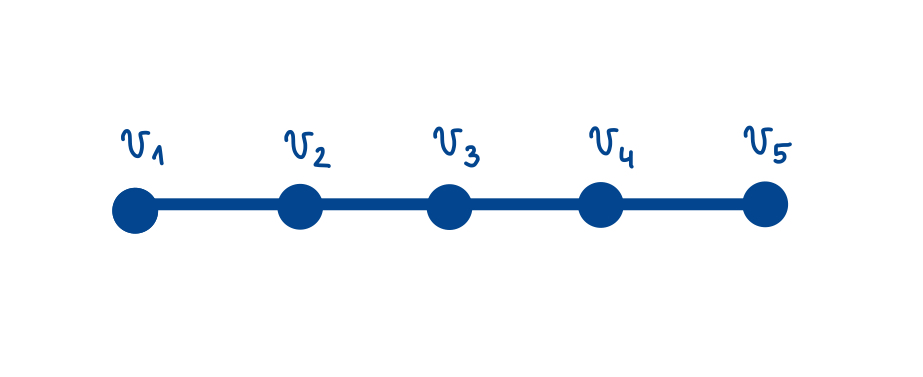
\includegraphics[width=0.6\textwidth]{IMG_pot.jpg}
    \label{fig:pot}      
\end{figure}

\end{primer}


\begin{primer}\label{primer_2.5.}
    Označimo vozlišča cikla z $v_1, v_2, ..., v_n$, kot je prikazano na sliki \ref{fig:cikel}. 
    Izberimo podmnožico $W = {v_1, v_2} \subseteq V(G).$ Metrične predstavitve vozlišč grafa $C_n$, 
    glede na izbrano podmnožico vozlišč, so potem sledeče:
    \begin{align*}
        r_W(v_1) = (d(v_1, v_1), d(v_1, v_2)) & = (0, 1) \\
        r_W(v_2) = (d(v_2, v_1), d(v_2, v_2)) & = (1, 0) \\
        r_W(v_3) = (d(v_3, v_1), d(v_3, v_2)) & = (2, 1) \\
        r_W(v_4) = (d(v_4, v_1), d(v_4, v_2)) & = (3, 2) \\
        & \dots \\
        r_W(v_{n-1}) = (d(v_{n-1}, v_1), d(v_{n-1}, v_2)) & = (2, 3) \\
        r_W(v_n) = (d(v_n, v_1), d(v_n, v_2)) & = (1, 2)
    \end{align*}
    
    Zopet vidimo, da so metrične predstavitve vseh vozlišč med seboj različne. Če bi vzeli 
    množico $W \setminus \{v_i\}$, bi imeli po dve vozlišči enako metrično prestavitev.
    $W$  je torej najmanjša rešljiva množica, njena velikost pa je enaka $2$. Metrična 
    dimenzija poljubno velikega cikla je enaka $\beta(C_n) = 2.$

    \begin{figure}[h]
        \caption{Graf $C_5$.}
        \centering
        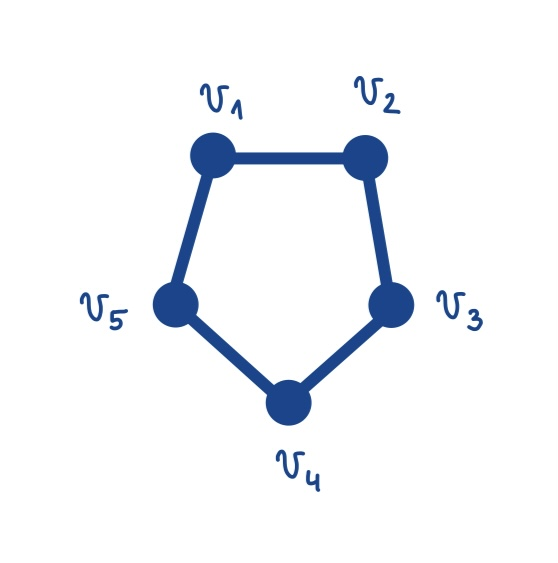
\includegraphics[width=0.4\textwidth]{IMG_cikel.jpg}
        \label{fig:cikel}
    \end{figure}

\end{primer}

\begin{primer}\label{primer_2.6.}
    Označimo vozlišča polnega grafa z $v_1, v_2, ..., v_n$, kot je prikazano na sliki \ref{fig:polni}. 
    Izberimo podmnožico $W = {v_1, v_2, ... , v_{n-1}} \subseteq V(G).$ 
    Metrične predstavitve vozlišč grafa $K_n$, glede na izbrano podmnožico vozlišč, so potem 
    sledeče:
    \begin{align*}
        r_W(v_1) = (d(v_1, v_1), d(v_1, v_2), ... , d(v_1, v_{n-1})) & = (0, 1, ... , 1) \\
        r_W(v_2) = (d(v_2, v_1), d(v_2, v_2), ... , d(v_2, v_{n-1})) & = (1, 0, ... , 1) \\
        & \dots \\
        r_W(v_{n-1}) = (d(v_{n-1}, v_1), d(v_{n-1}, v_2), ... , d(v_{n-1}, v_{n-1})) & = (1, 1, ... , 0) \\
        r_W(v_n) = (d(v_n, v_1), d(v_n, v_2), ... ,  d(v_n, v_{n-1})) & = (1, 1, ... , 1)
    \end{align*}
    
    Zopet vidimo, da so metrične predstavitve vseh vozlišč med seboj različne. Vsako 
    vozlišče ima na $i$ - ti komponenti $0$ in povsod drugje $1$, z izjemo vozlišča $v_n$, 
    ki ima povsod $1$. Če bi vzeli poljubno $W \setminus \{v_i\}$, bi imeli vozlišči $v_i$ 
    in $v_n$ enaki metrični predstavitvi. $W$  je torej najmanjša rešljiva množica, njena 
    velikost pa je enaka $n-1$. Metrična dimenzija poljubno velikega cikla je enaka $\beta(K_n) = n-1.$

    \begin{figure}[h]
        \caption{Graf $K_5$.}
        \centering
        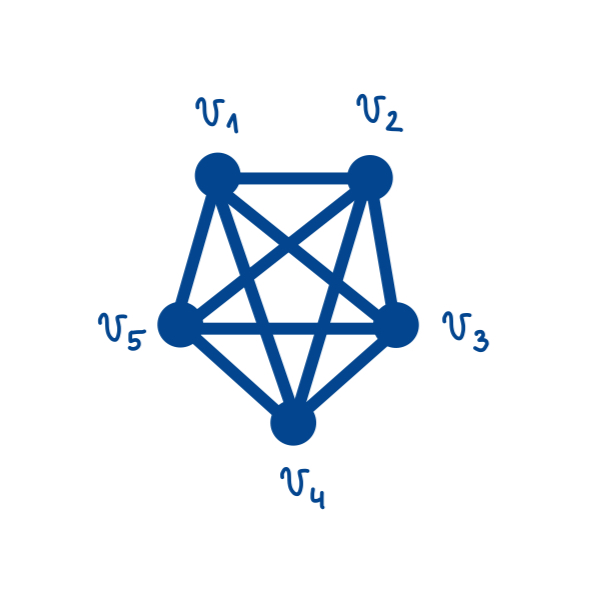
\includegraphics[width=0.4\textwidth]{IMG_polni.jpg}
        \label{fig:polni}
    \end{figure}

\end{primer}


%%%%%%%%%%%%%%%%%%%%%%%%%%%%%%%%%%%%%%%%%%%%%%%%%%%%%%%%%%%%%%%%%%%%%%%%%%%%%%%
%%%%%%%%%%%%%%%%%%%%%%%%%%%%%%%%%%%%%%%%%%%%%%%%%%%%%%%%%%%%%%%%%%%%%%%%%%%%%%%
%%%%%%%%%%%%%%%%%%%%%%%%%%%%%%%%%%%%%%%%%%%%%%%%%%%%%%%%%%%%%%%%%%%%%%%%%%%%%%%
%%%%%%%%%%%%%%%%%%%%%%%%%%%%%%%%%%%%%%%%%%%%%%%%%%%%%%%%%%%%%%%%%%%%%%%%%%%%%%%


\subsection{Lastnosti}

Nekaj osnovnih ugotovitev o rešljivih množicah grafa lahko razberemo iz zgornjih primerov.

\begin{trditev} \label{trditev_2.8.}
Za povezan graf $G$, je $V(G)$ rešljiva množica.
\end{trditev}

\begin{dokaz}
Predpostavimo $|V(G)|= n$. Označimo vozlišča z $v_1, ..., v_n$.
Za posamezno vozlišče bo metrična predstavitev sledeča:
$$r_{V(G)}(v_k) = (d(v_k, v_1), ..., d(v_k, v_k), ... , d(v_k, v_n)) = (d(v_k, v_1), ..., 0 , ... , d(v_k, v_n)).$$
Torej za vsako vozlišče $v_k$ bo $k$-ta komponenta metrične predstavitve enaka $0$. 
Zaradi \ref{nicelna_razdalja} je to tudi edina komponenta v vektorju, ki bo enaka $0$.
Sledi $\forall u, v \in V(G): u \neq v \Rightarrow r_{V(G)}(v) \neq r_{V(G)}(u)$, 
torej je $V(G)$ rešljiva množica.
\end{dokaz}

% a je sploh definirana razdalja na nepovezanem grafu?? s bi se dalo narest kakšno smiselno razširitev??
%iz te trditve sledi, da metrična dimenzija vselej obstaja in je manjša ali enaka |V(G)|.

\begin{trditev}
    Rešljiva baza povezanega grafa $G$ ni enolično določena.
\end{trditev}
\begin{dokaz}
    To hitro vidimo na primeru \ref{primer_2.4.}.
    Za $W$ bi lahko vezli tudi vozlišče $v_n$ in prišli do enakega rezultata.
\end{dokaz}

V defnicijah \ref{def:1} in \ref{def:2} smo prepostavili, da imamo neprazno podmnožico 
vozlišč. Če bi vzeli prazno množico, bi bila definicija metrične dimenzije nesmiselna. 
Iz trditve \ref{trditev_2.8.} lahko potem sklepamo, da metrična dimenzija za graf vselej 
obstaja in lahko zapišemo naslednjo posledico:

\begin{posledica}
    Za povezan graf $G$ velja 
    $$1 \leq \beta(G) \leq |V(G)| - 1. $$
\end{posledica}
\begin{dokaz}
    Iz definicije \ref{def:3} sledi $1 \leq \beta(G)$. Iz trditve \ref{trditev_2.8.} 
    pa sledi $\beta(G) \leq |V(G)|.$ Predpostavimo $|V(G)| = n$ in $V(G) = \{ v_1, ... , v_n\}$. 
    Vzemimo sedaj podmnožico $W = \{ v_1, ... , v_{n-1}\}.$
    Metrične predstavitve vozlišč glede na $W$ so sledeče:

    \begin{align*}
        r_W(v_1) & = (0, d(v_1, v_2), ..., d(v_1, v_k), ... , d(v_1, v_{n-1})) \\
        r_W(v_2) & = (d(v_2, v_1), 0, ..., d(v_2, v_k), ... , d(v_2, v_{n-1})) \\
        & \dots \\
        r_W(v_k) & = (d(v_k, v_1), d(v_k, v_2), ..., 0 , ... , d(v_k, v_{n-1})) \\
        & \dots \\
        r_W(v_{n-1}) & = (d(v_{n-1}, v_1), d(v_{n-1}, v_2), ... , d(v_{n-1}, v_k) , ..., 0) \\
        r_W(v_n) & = (d(v_n, v_1), d(v_n, v_2), ...,  d(v_n, v_k), ... , d(v_n, v_{n-1})) \\
    \end{align*}
    Vidimo, da so vse metrične predstavitve med seboj različne, torej je $W$ rešljiva in 
    $\beta(G) \leq n - 1.$ 
\end{dokaz}

\begin{trditev} \label{trditev_2.10.}
    Naj bo $G$ povezan graf in $|V(G)| = n \geq 2.$ Potem velja:
    \begin{enumerate}
        \item $G = K_n \; \Leftrightarrow \; \beta(G) = n - 1.$
        \item $G = P_n \; \Leftrightarrow \; \beta(G) = 1.$
    \end{enumerate} 
\end{trditev}

\begin{dokaz}
    Implikacijo v desno stran za obe točki smo že pokazali v primerih \ref{primer_2.4.} in 
    \ref{primer_2.6.}.
    \begin{enumerate}
        \item $\Leftarrow$  TODO
        \item $\Leftarrow$
        Recimo, da imamo povezan graf $G$ na $n$ vozliščih z $\beta(G) = 1.$ Sledi, da obstaja neka 
        rešljiva baza $W = \{ w \}.$ Označimo $V(G) = \{ v_1, v_2, ... , v_{n-1}, w\}.$ Sedaj mora 
        veljati, da so števila 
        $$ d(v_1, w),  d(v_2, v_1), ..., d(v_{n-1}, w), d(w, w) $$
        paroma različna. Vemo $d(w, w) = 0$. Ker je $G$ povezan, mora obstajati vsaj eno vozlišče, 
        ki je sosednje z $w$. BSŠ naj bo $v_{n-1} \sim w$. Torej je $d(v_{n-1}, w) = 1$ in sledi, 
        da nobeno drugo vozlišče ni sosednje z $w$. Zopet zaradi povezanosti grafa obstaja vozlišče 
        sosednje z $v_{n-1},$ ki je različno od $w$. Recimo, da je to $v_{n-2}$, za katerega sedaj 
        velja $d(v_{n-2}, w) = 2.$ Spet je to edino takšno vozlišče. Nadaljujemo podobno, 
        dokler ne pridemo do $v_1.$ Dobimo graf $P_n.$
    \end{enumerate}
\end{dokaz}

%Konec koncev je vsega konec.%
%Začetki so najtežji.%


%%%%%%%%%%%%%%%%%%%%%%%%%%%%%%%%%%%%%%%%%%%%%%%%%%%%%%%%%%%%%%%%%%%%%%%%%%%%%%%
%%%%%%%%%%%%%%%%%%%%%%%%%%%%%%%%%%%%%%%%%%%%%%%%%%%%%%%%%%%%%%%%%%%%%%%%%%%%%%%


\subsubsection{Metrična dimenzija in premer grafa}

Ni presenetljivo, da lahko najdemo povezavo med metrično dimenzijo in premerom grafa.
Spomnimo se matematične definicije premera.

\begin{definicija}
    Premer grafa $G$ označujemo z ${\rm diam}(G)$ in je enak dolžini najdaljše najkrajše 
    poti v grafu. Torej $${\rm diam}(G) = \underset{v, u \in V(G)}{\max} d(u, v).$$
\end{definicija}

\begin{trditev}
    Naj bo $G$ povezan graf in $|V(G)| = n$. Potem velja naslednja povezava:
    $$n \leq ({\rm diam}(G))^{\beta (G)} + \beta (G). $$
\end{trditev}

\begin{dokaz}
    Naj bo $R$ rešljiva baza grafa $G$, torej $|R| = \beta(G).$ Zanima nas, največ koliko 
    vozlišč ima lahko tak graf $G$. Vozlišča iz množice $R$ bodo imela natanko eno 
    komponento metrične predstavitve enako nič, tako se bodo te razlikovale med sabo in 
    vseh ostalih. Če pa vzamemo vozlišče $v \notin R$, pa velja sledeče:
    $$\forall r_i \in R: 1 \leq d(v, r_i) \leq {\rm diam}(G).$$
    
    Vseh možnih različnih metričnih predstavitev za vozlišča izven rešljive množice $R$ 
    je tako $({\rm diam}(G))^{\beta (G)}$
    in lahko zapišemo:
    $$n \leq ({\rm diam}(G))^{\beta (G)} + \beta (G).$$
\end{dokaz}

V resnici lahko red grafa z dano metrično dimenzijo in premerom še bolj omejimo.

\begin{trditev}
    Naj bo $G$ povezan graf in $|V(G)| = n$. Označimo $ \delta = {\rm diam}(G)$ in 
    $\beta = \beta (G)$. Potem velja

    $$n \leq \Bigl ( \Bigl \lfloor {\frac{2 \delta}{3}}\Bigr \rfloor + 1 \Bigr )^{\beta} + 
    \beta \sum_{i = 1}^{\lceil \delta /3 \rceil} {(2i - 1)^{\beta - 1}}. $$
\end{trditev}

\begin{dokaz}
    TODO
\end{dokaz}

Ta zgornja meja postane še bolj natančna za posamezne družine grafov, vendar v tem delu
tega ne bomo obravnavali tako podrobno.


%%%%%%%%%%%%%%%%%%%%%%%%%%%%%%%%%%%%%%%%%%%%%%%%%%%%%%%%%%%%%%%%%%%%%%%%%%%%%%%
%%%%%%%%%%%%%%%%%%%%%%%%%%%%%%%%%%%%%%%%%%%%%%%%%%%%%%%%%%%%%%%%%%%%%%%%%%%%%%%


\subsubsection{Dvojčki in metrična dimenzija}
Spomnimo se pojma soseščine vozlišča.

\begin{definicija}
    Naj bo $G$ povezan graf in $v \in V(G)$ vozlišče na grafu. Množico 
    $$N(v) = \{u \in V(G) \, | \,vu \in E(G) \}$$ imenujemo soseščina vozlišča $v$.
\end{definicija}

Sedaj vpeljimo ekvivalenčno relacijo na vozliščih
$$v \equiv u \Leftrightarrow N(v)\setminus \{u\} = N(u) \setminus \{v\}$$
Če sta vozlišči v tej ekvivalenčni relaciji, pravimo, da sta dvojčka. 
Ekvivalenčni razred vozlišča $v$ označimo z $v^{*}$, 
množico vseh ekvivalenčnih razredov z $\tau (G)$, število vseh razredov pa naj bo označeno 
z $|\tau(G)| = \iota(G).$

\begin{lema}
    Naj bosta $u, v \in v(G)$ dvojčka. Potem je 
    $$\forall w \in V(G) \setminus \{u, v\} : d(u, w) = d(v, w).$$
\end{lema}

\begin{dokaz}
    Naj bosta $u$ in $v$ dvojčka v grafu $G$. Označimo $V(G) = \{u, v, w_1, ..., w_k\}$ 
    in $S = N(v)\setminus \{u\} = N(u) \setminus \{v\}$. Izberimo vozlišče 
    $w_i \in V(G) \setminus \{u, v\}.$
    \begin{enumerate}
        \item $w_i \in S \; \Rightarrow \; d(u, w_i) = d(v, w_i) = 1.$
        \item $w_j \notin S \; \Rightarrow \; d(u, w_j) = m \geq 2$. 
    
        Denimo $m=2.$ Potem obstaja $w_j \in S,$ da je $w_j \sim w_i$ in sledi $d(v, w_i) = 2.$
        
        Naj bo sedaj $m > 2.$ Obstaja vozlišče $w_j,$ sosednje od $w_i$, za katerega velja 
        $d(u, w_j) = m-1.$ Potem je po indukcijski predpostavki tudi $d(v, w_j) = m-1$ in 
        sledi $d(v, w_i) = m-1 + 1 = m.$
    \end{enumerate}
    
\end{dokaz}

Iz tega sledi, da mora vsaka rešljiva množica vsebovati vsaj enega od dvojčkov.
Zapišemo lahko naslednjo trditev:

\begin{trditev}
    Za povezan graf $G$ velja
    $$\beta(G) \geq \sum_{v^{*} \in \tau(G)} (|v^{*}| - 1).$$
\end{trditev}

\begin{dokaz}
    TODO
\end{dokaz}

\subsection{NP - poln problem}
TODO


%%%%%%%%%%%%%%%%%%%%%%%%%%%%%%%%%%%%%%%%%%%%%%%%%%%%%%%%%%%%%%%%%%%%%%%%%%%%%%%
%%%%%%%%%%%%%%%%%%%%%%%%%%%%%%%%%%%%%%%%%%%%%%%%%%%%%%%%%%%%%%%%%%%%%%%%%%%%%%%
%%%%%%%%%%%%%%%%%%%%%%%%%%%%%%%%%%%%%%%%%%%%%%%%%%%%%%%%%%%%%%%%%%%%%%%%%%%%%%%
%%%%%%%%%%%%%%%%%%%%%%%%%%%%%%%%%%%%%%%%%%%%%%%%%%%%%%%%%%%%%%%%%%%%%%%%%%%%%%%


\section{Leksikografski produkt grafov}



\begin{definicija}
    Leksikografski produkt $G[H]$ grafov $G$ in $H$ je definiran na množici vozlišč 
    $V (G[H]) = V (G)\times V (H)$. Dve različni vozlišči $(u, v)$ in $(x, y)$ sta 
    sosedni, kadar velja
\begin{itemize}
    \item $ux \in E(G)$ ali
    \item $u = x$ in $vy \in E(H).$ 
\end{itemize}
\end{definicija}


%%%%%%%%%%%%%%%%%%%%%%%%%%%%%%%%%%%%%%%%%%%%%%%%%%%%%%%%%%%%%%%%%%%%%%%%%%%%%%%
%%%%%%%%%%%%%%%%%%%%%%%%%%%%%%%%%%%%%%%%%%%%%%%%%%%%%%%%%%%%%%%%%%%%%%%%%%%%%%%


\subsection{primer}
Za lažjo predstavo si lahko ogledamo sliko \ref{fig:produkt}, ki prikazuje leksikografski produkt
dveh naključnih povzeanih grafov.

\begin{figure}[h]
    \caption{Leksikografski produkt poljubnih povezanih grafov $G$ in $H$.}
    \centering
    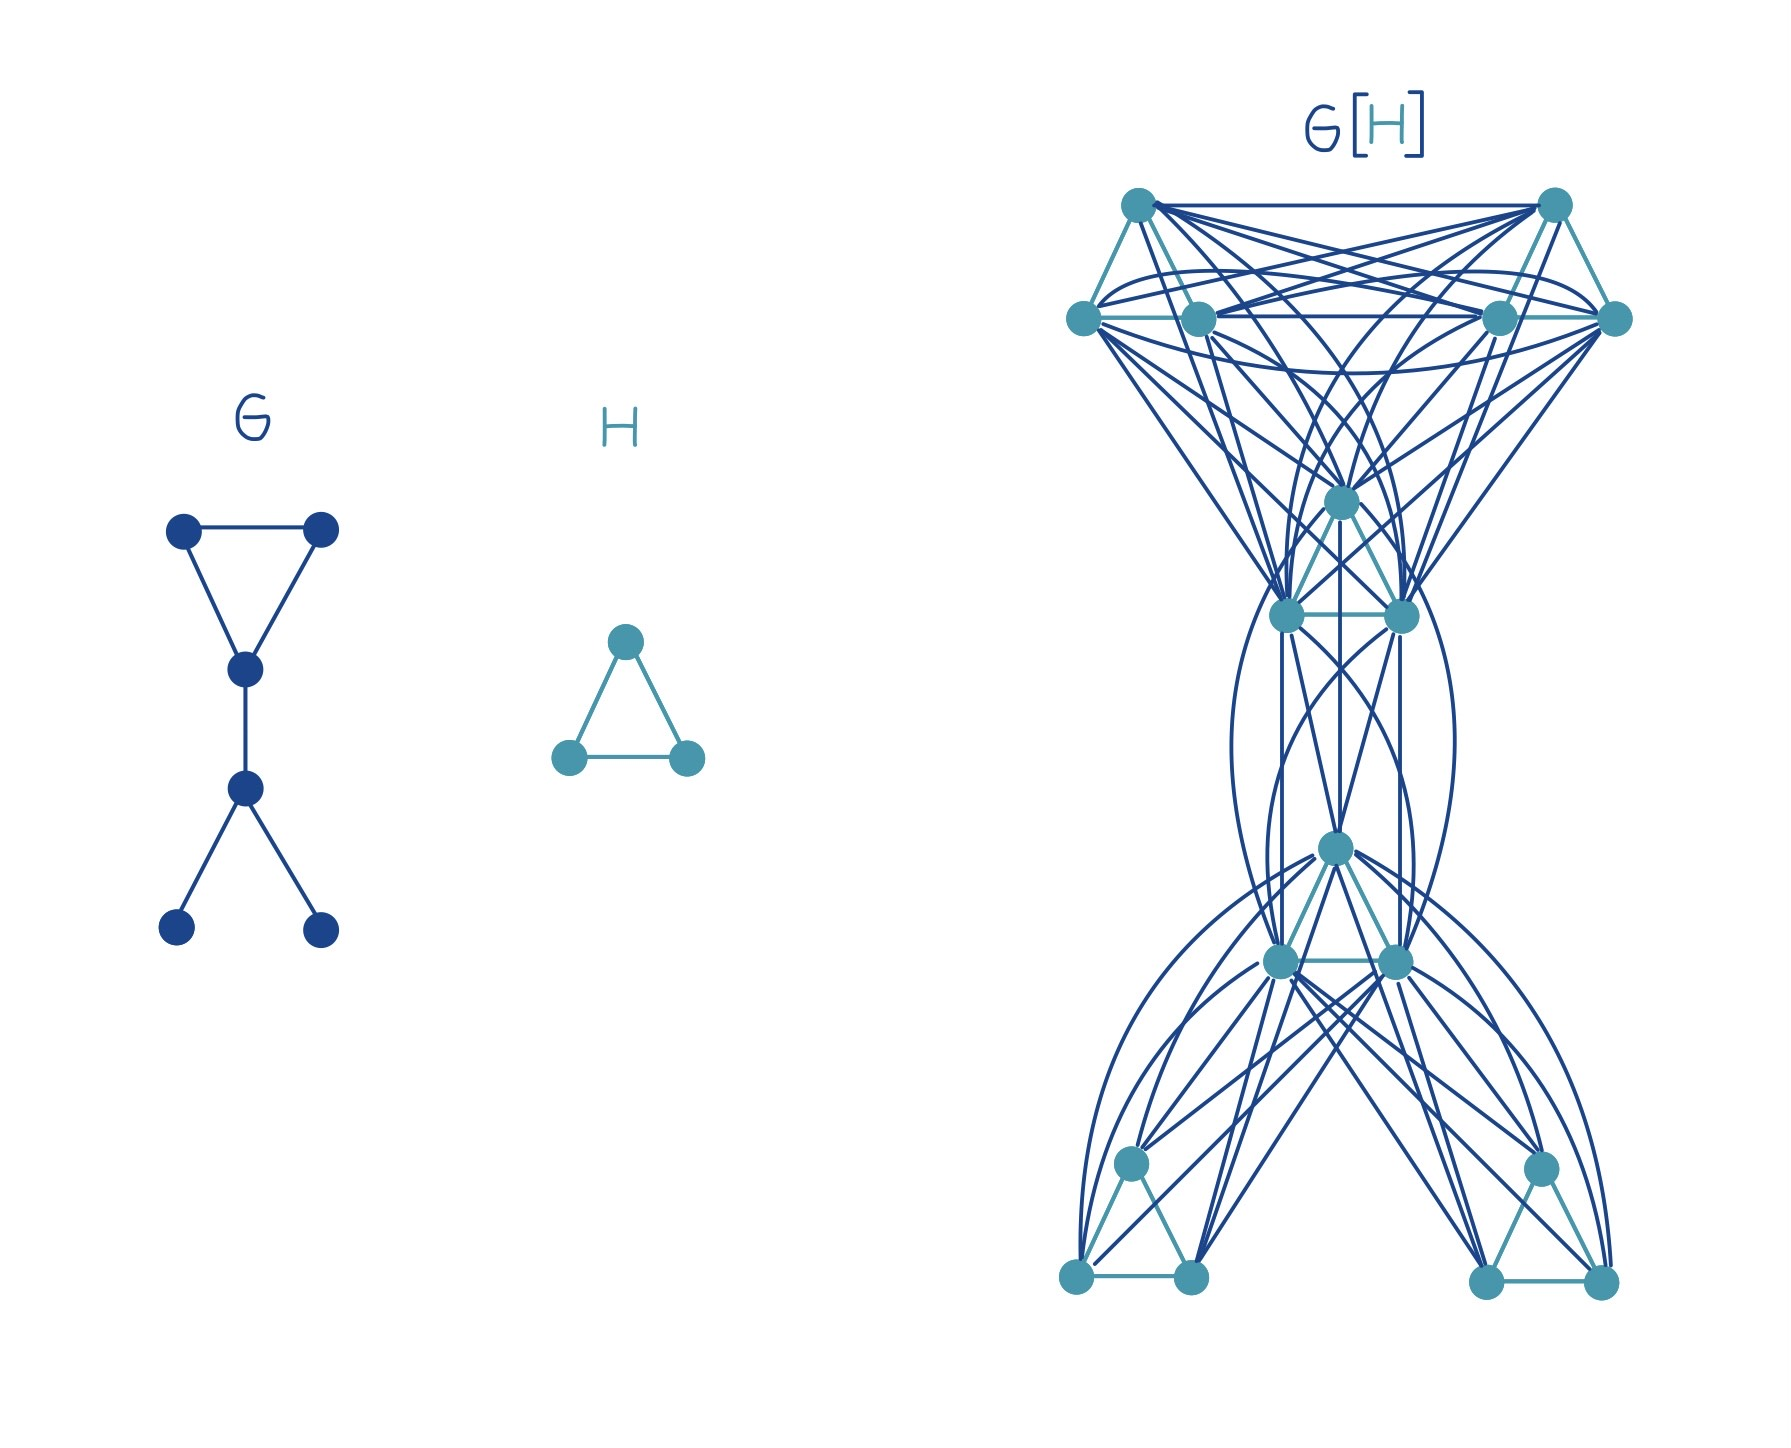
\includegraphics[width=\textwidth]{IMG_produkt.jpg}   
    \label{fig:produkt}   
\end{figure}


%%%%%%%%%%%%%%%%%%%%%%%%%%%%%%%%%%%%%%%%%%%%%%%%%%%%%%%%%%%%%%%%%%%%%%%%%%%%%%%
%%%%%%%%%%%%%%%%%%%%%%%%%%%%%%%%%%%%%%%%%%%%%%%%%%%%%%%%%%%%%%%%%%%%%%%%%%%%%%%


\subsection{lastnosti}
Nekaj osnovnih lastnosti leksikografskega produkta grafov:
\begin{itemize}
    \item POVEZANOST: Če je $G$ povezan graf, potem je $G[H]$ povezan. 
    \item NEKOMUTATIVNOST: v splošnem velja $G[H] \neq H[G].$
    \item DISTRIBUTIVNOST: $(G_1 + G_2)[H] = G_1[H] + G_2[H],$ 
    \item ENAKOST KOMPLEMENTOV: $\overline{G[H]} = \overline{G} [\overline{H}].$
    % kako bi se v resnici pravilno reklo tej lastnosti...?
\end{itemize}

Poglejmo si kako izgleda razdalja med vozliščema v leksikografskem prodkutu grafov. 
Označimo preslikavo  $a: V(G) \times V(G) \rightarrow \mathbb{N};$   
$$ a(v, w) = \begin{cases}
    0; & v = w \\
    1; & v \sim w \\
    2; & v \not\sim w
\end{cases} 
$$ 
Opazujemo Leksikografski produkt povezanega grafa $G$ reda $n$, z množico vozlišč
$V(G) = \{v_1, v_2, ... , v_n \}$ in grafa $H$ reda $m$, z množico vozlišč 
$V(H) = \{u_1, u_2, ... , u_m \}$. Zaradi boljše preglednosti vpeljimo oznako 
$v_{ij} := (v_i, u_j) \in V(G[H]).$
Sedaj lahko zapišemo
$$
d_{G[H]}(v_{ij}, v_{rs}) = \begin{cases}
        d_G(v_i, v_r); & v_i \neq v_r \\
        a_H(u_j, u_s); & \text{sicer}
    \end{cases}
$$ 


%%%%%%%%%%%%%%%%%%%%%%%%%%%%%%%%%%%%%%%%%%%%%%%%%%%%%%%%%%%%%%%%%%%%%%%%%%%%%%%
%%%%%%%%%%%%%%%%%%%%%%%%%%%%%%%%%%%%%%%%%%%%%%%%%%%%%%%%%%%%%%%%%%%%%%%%%%%%%%%
%%%%%%%%%%%%%%%%%%%%%%%%%%%%%%%%%%%%%%%%%%%%%%%%%%%%%%%%%%%%%%%%%%%%%%%%%%%%%%%
%%%%%%%%%%%%%%%%%%%%%%%%%%%%%%%%%%%%%%%%%%%%%%%%%%%%%%%%%%%%%%%%%%%%%%%%%%%%%%%


\section{Metrična dimenzija leksikografskega produkta grafov}
 

%%%%%%%%%%%%%%%%%%%%%%%%%%%%%%%%%%%%%%%%%%%%%%%%%%%%%%%%%%%%%%%%%%%%%%%%%%%%%%%
%%%%%%%%%%%%%%%%%%%%%%%%%%%%%%%%%%%%%%%%%%%%%%%%%%%%%%%%%%%%%%%%%%%%%%%%%%%%%%%


\subsection{Metrična dimenzija in komponente}
Obravnavamo leksikografski produkt $G[H]$, kjer je $G$ povezan graf in $H$ pojuben 
graf. Naj bosta $a \in V(G)$ in $b \in H$ poljubni vozlišči. Za potrebe tega 
podpoglavlja vpeljimo naslednje oznake:
\begin{itemize}
    \item $H(a) = \{ (a, v) \; | \; v \in V(H) \}$.
    \item $G(b) = \{ (v, b) \; | \; v \in V(G) \}$.
    \item Če so $H_1, H_2, ..., H_k$ komponente grafa $H$, označimo 
    $H_i(a) = \{ (a, v) \; | \; v \in V(H_i) \}$
\end{itemize}

Vzemimo sosednji vozlišči $a$, $b \in V(G)$. Vemo, da je vsako vozlišče iz $H(b)$ 
sosednje vsakemu iz $H_i(a).$ 
Hitro lahko preverimo, da je inducirani podgraf grafa $G[H]$, kjer vzamemo eno 
vozlišče iz množice $H(b)$ in vsa vozlišča iz $H_i(a)$, izomorfen grafu $H_i + K_1.$ 
S pomočjo rešljive baze tega združenega grafa bomo konstruirali rešljivo bazo $G[H]$.

\begin{lema}
    Naj bo $Q$ povezan graf. Obstaja rešljiva baza $S$ grafa $Q + K_1,$ da je 
    $S \subseteq V(Q).$
\end{lema}

\begin{dokaz}
    Združitev grafov $Q + K_1$ ima množico vozlišč $V(Q) \cup \{ v \}.$ Naj bo $S$ 
    rešljiva baza $Q + K_1$. Če $v \notin S.$ je lema dokazana. Denimo $v \in S.$ 
    V tem primeru ločimo dve situaciji:
    \begin{enumerate}
        \item $S\ \{ v \} = \emptyset \; \Rightarrow \;$   
    \end{enumerate}
\end{dokaz}



%%%%%%%%%%%%%%%%%%%%%%%%%%%%%%%%%%%%%%%%%%%%%%%%%%%%%%%%%%%%%%%%%%%%%%%%%%%%%%%
%%%%%%%%%%%%%%%%%%%%%%%%%%%%%%%%%%%%%%%%%%%%%%%%%%%%%%%%%%%%%%%%%%%%%%%%%%%%%%%


\subsection{Metrična dimenzija, sosedska dimenzija in dvojčki}


%%%%%%%%%%%%%%%%%%%%%%%%%%%%%%%%%%%%%%%%%%%%%%%%%%%%%%%%%%%%%%%%%%%%%%%%%%%%%%%
%%%%%%%%%%%%%%%%%%%%%%%%%%%%%%%%%%%%%%%%%%%%%%%%%%%%%%%%%%%%%%%%%%%%%%%%%%%%%%%


\subsection{Povezave in skupni rezultati??}
%če mi to rata sem car.


% \section{...}
% ...

% \section{Zaključek}
% ...

\end{document}
